\chapter{Core Systems Design}
\label{cha:core_system_design}
\section{Requirements Analysis}
\subsection{User Requirements}
The following user requirements for the system were gathered by inspecting similar systems, personal creativity and feedback from supervisor or wearables lab team. User stories were chosen for representation.
\subsection{Functional Requirements}
\subsection{Non-Functional Requirements}
\section{High-level overview}
\begin{figure}
    \centering
    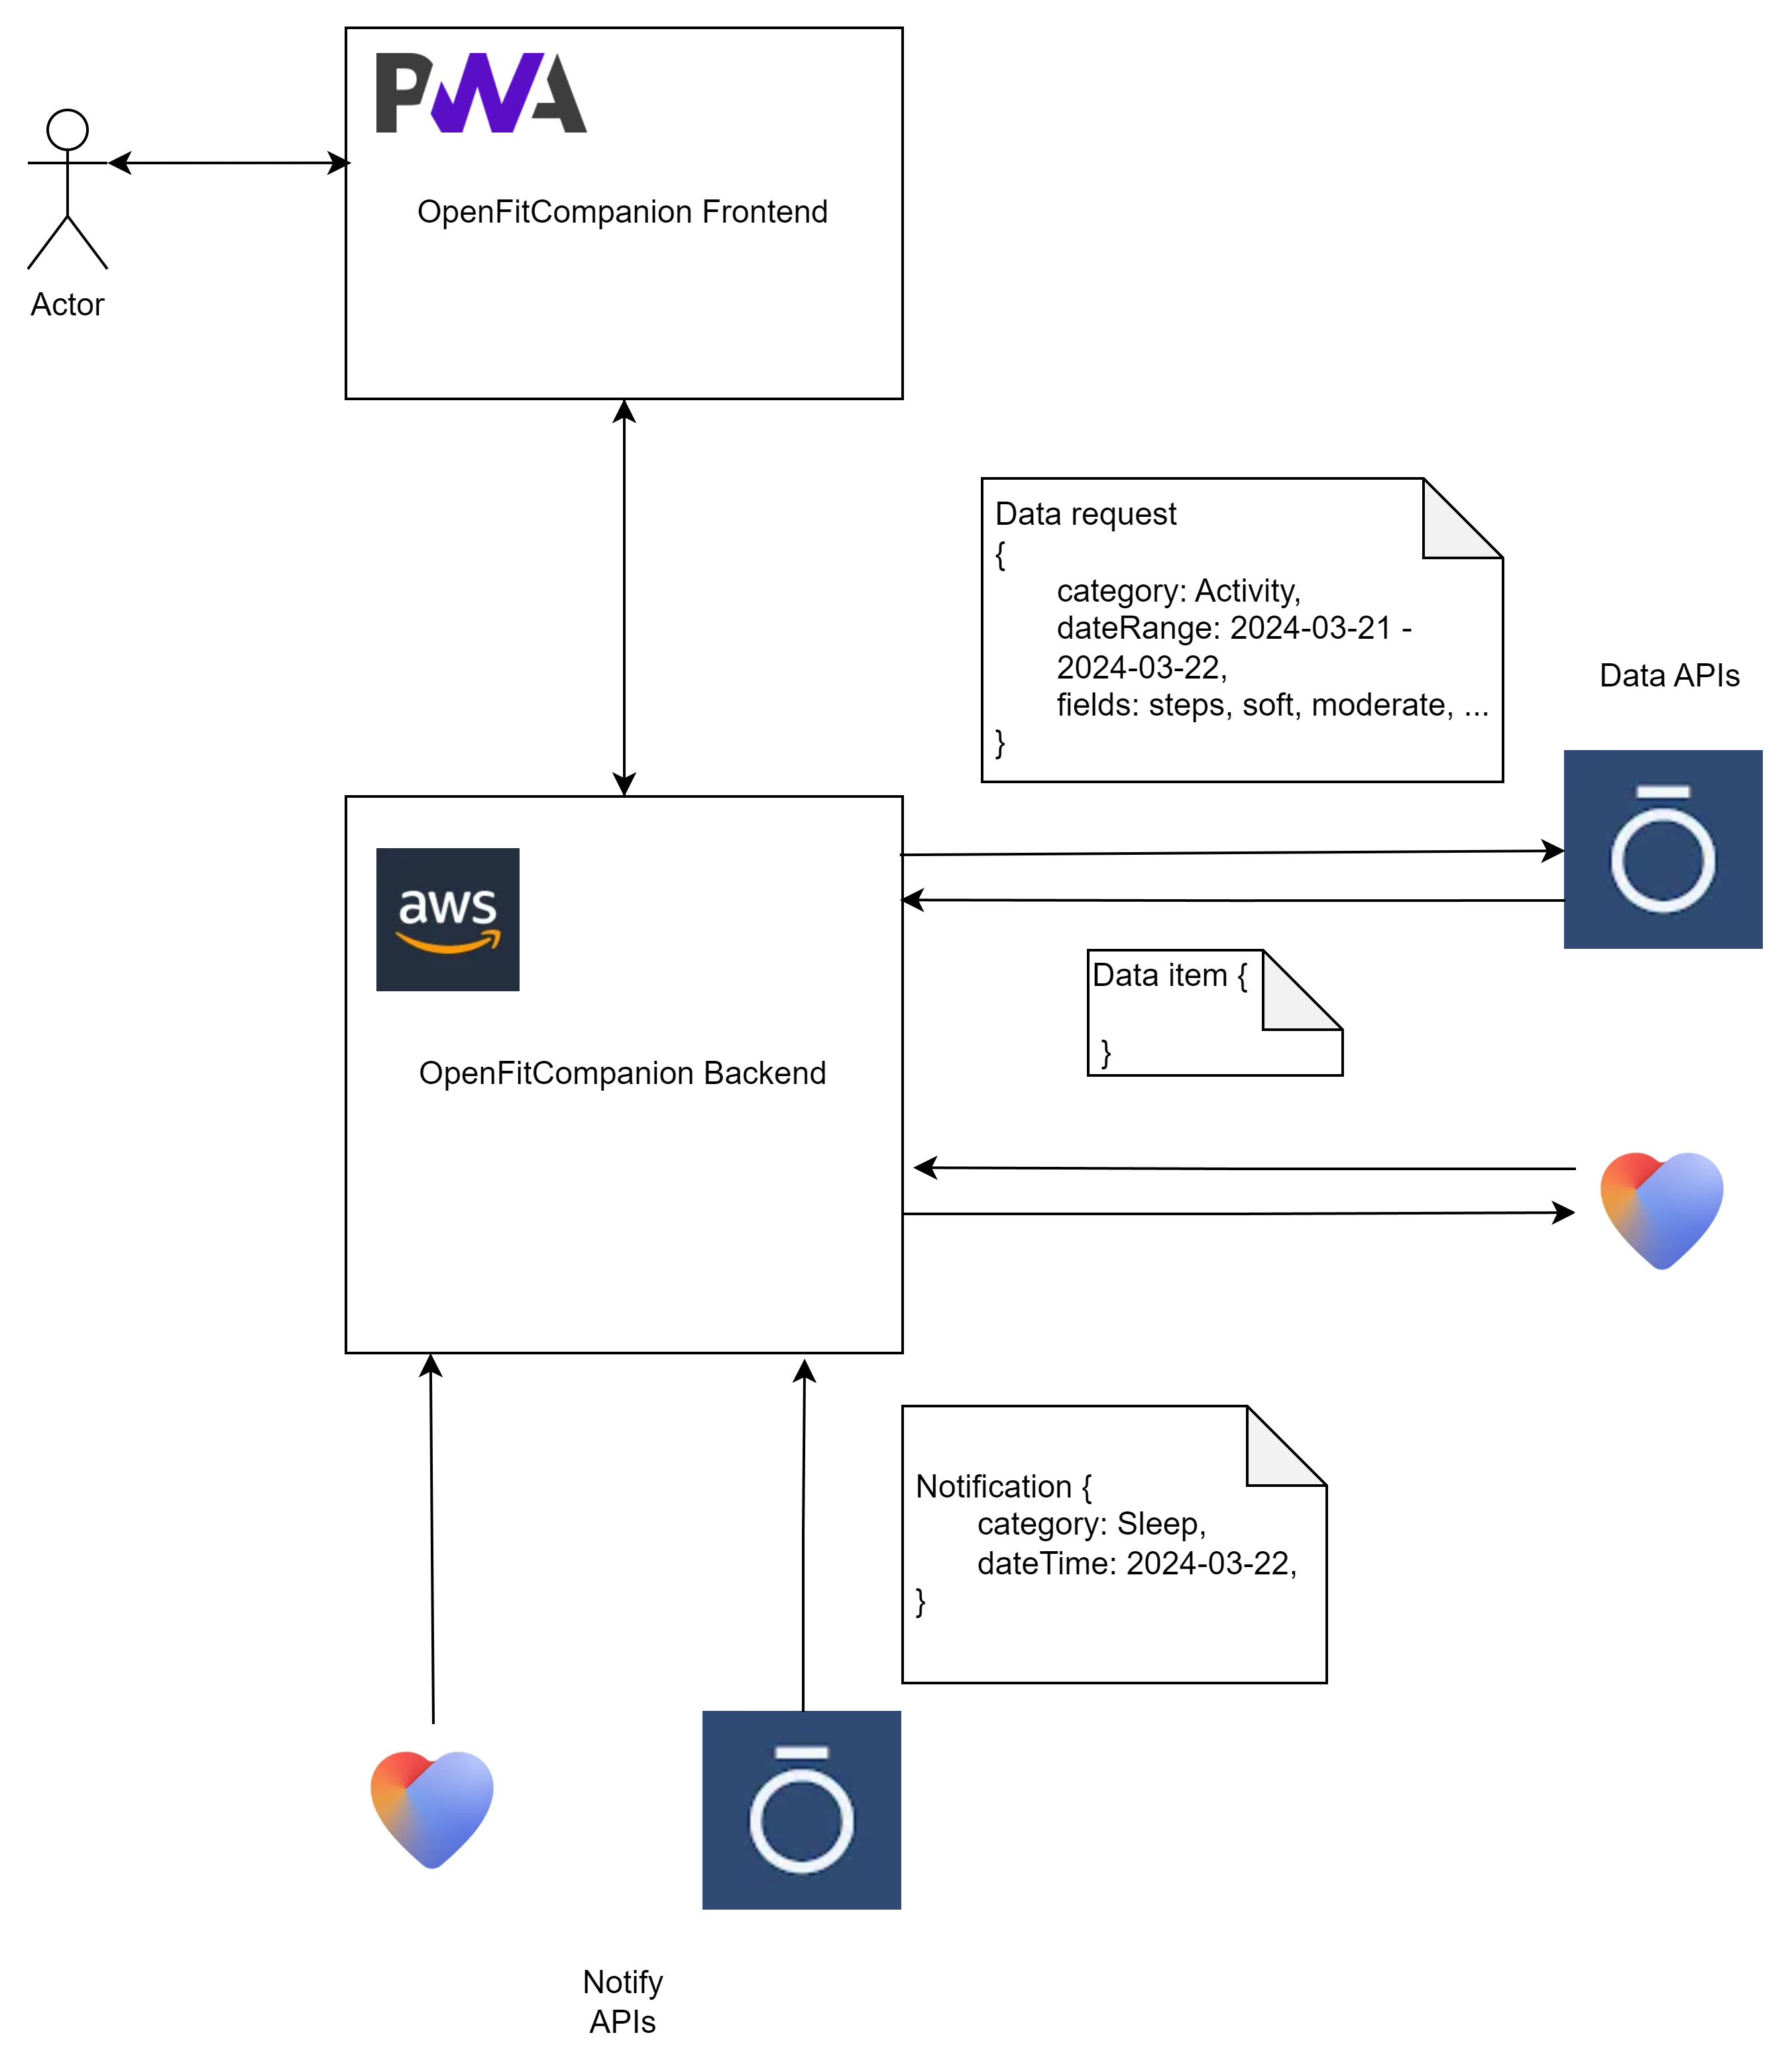
\includegraphics[width=\textwidth,height=\textheight,keepaspectratio]{images/highLevel.png}
    \caption{High-Level architecture diagram}
    \label{fig:1}
\end{figure}
Overall, the architecture is considered event-driven. Computation only needs to happen in response to an external event. This is enabled by providers providing Webhook integrations. Essentially, the backend gets a notification from providers whenever there is new data available from them. The following is the diagram together with sample data exchanged: \ref{fig:1}

Cloud deployed backend service receives notifications from providers, containing information that allows atomic processing of that notification. It does not matter what other requests came before or if any are executing at the moment. 

In response to the notification, backend sends a request to Data APIs of providers, receiving an item(s) back and finally persisting it in a database for further purposes. 

Withings and Oura providers were integrated at the time of this report. However, the system can scale to many more providers. The only requirement for a provider is that they have Data API we can use. Even if a particular provider did not have a webhook (notification) service, we could re-sync with data APIs on regular schedule, like every 30 minutes. With the interval value being a trade-off between potentially more latency in syncing the data or wasted compute time when there are no updates. This would be quite costly if the system was publicly available service, as that scheduled request would be needed for each user. However, for our use case of self-deployed service, the cost would be negligible. However, there is still reliance on provider's API services to get the actual data from devices. System does not communicate with the smart devices directly via Bluetooth, there is an intermediate provider's system that data must be pass through. So, if a provider does not have such service, we can't integrate their devices into the system. However, all providers examined at least provided Google Fit integration, from which the data could be fetched instead. 

Ultimately, the data is transformed into useful information (insight) using using LLMs and classical algorithms. This is then presented to the user through the frontend. 
\begin{itemize}
    \item {Dashboard, contains a graph visualizing data from all devices, allowing for comparison and a brief overview of trends.}
    \item {Daily Report, containing a graph visualizing MET minutes completed this week and the goal MET minutes per week; Feedback on expected activity completion for that day and AI feedback for that day. Provides the user with information, allowing them to reflect on their day, seeing the progress towards fulfilling the weekly activity goal. A notification is sent to the user when such report is available. This constitutes Type 2 nudge, as it  engages user's conscious, reflective thinking to get them more motivated for physical activity tomorrow. However, there is also a component of Type 1 nudge with report notifications being opt-out rather than opt-in.}
    \item {Weekly Report, focusing more on consistency rather than absolute values and goal completions. Contains a graph visualizing deviation from the mean value of daily activity or sleep score. Same nudging as Daily Report.}
    \item {Activity plan, containing curated list of planned physical activities for the day, generated by AI. Also containing feedback about activity minutes done today. Similarly, it has type 1 nudging factor, being opt-out as well as Type 2 nudging, by notifying users at certain times when they should be doing exercises, and providing well-suited list of exercises, with description of benefits and video examples on how to perform them. This removes the need for user to plan their own workouts, removing decision paralysis. This imitates real-life coaching with a personal trainer, bringing benefits such as accountability and personalisation to users who may not be able to afford the real counterpart.}
\end{itemize}

\section{Back-end}
\subsection{AWS services}
\subsection{Adapters}
\subsection{Unifying}
\section{Front-end}
\subsection{UI}
\subsection{Notifying}
\subsection{Reporting}

TODO: Do this chapter
